\documentclass[assignment3.tex]{subfiles}
\begin{document}

\section*{1η Άσκηση}
Ζητείται το πολυώνυμο \textlatin{Lagrange} τετάρτου βαθμού που παρεμβάλει την $f(x)=e^{2x}-1$ στα σημεία $\lbrace1, 1.1, 1.2, 1.3,1.4\rbrace$. Η επίλυση αυτού το προβλήματος είναι απλή. Γίνεται εφαρμογή των εξισώσεων (\ref{eq:lagrange_ith}) και (\ref{eq:lagrange_poly}), με το αποτέλεσμα να δίνεται στο Σχήμα \ref{fig:ex1}.
\begin{equation}
L_i(x) = \prod_{j=0, j\neq i}^{4}\frac{x-x_j}{x_i-x_j}
\label{eq:lagrange_ith}
\end{equation}
\begin{equation}
p_4(x) = \sum_{i=0}^{4}L_i(x)f(x_i)
\label{eq:lagrange_poly}
\end{equation}
\begin{figure}[hp]
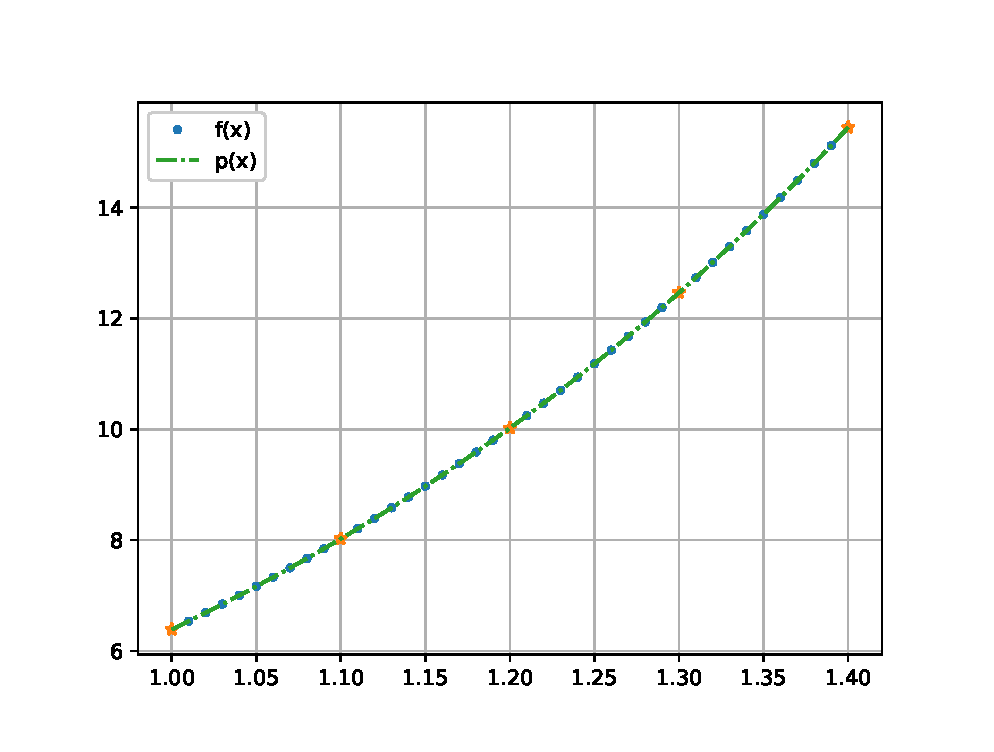
\includegraphics[width=0.9\textwidth]{ex1.eps}
\centering
\caption{Παρεμβολή με πολυώνυμο \textlatin{Lagrange}}
\label{fig:ex1}
\end{figure}
Η τιμή της συνάρτησης στο σημείο $x=1.25$ είναι $f(1.25)=11.1824939607$ ενώ η τιμή του πολυωνύμου είναι $p_4(1.25)=11.1824517251$. Παρατηρείται ότι η διαφορά των δύο τιμών είναι της τάξης του $10^{-5}$.

Παρακάτω ακολουθεί ο κώδικας που γράφτηκε σε \textlatin{Python} και έγινε χρήση της βιβλιοθήκης \textlatin{Numpy}.
\selectlanguage{english}
\lstinputlisting[style=python, firstline=8]{ex1.py}
\end{document}